\chapter{Введение}
\label{chap:intro}

В классическом однородном многоядерном планировании планировщик операционной системы распределяет доступные однородные ядра между динамически поступающими программами~\cite{Anderson2006}. Когда количество ожидающих выполнения программ превышает количество ядер, планировщик распределяет программы по приоритетам, либо по статическим приоритетам, установленным разработчиком системы, либо по конкретным динамически вычисляемым приоритетам. Целями планировщика являются минимизация среднего времени выполнения программ, задержки, числа миграций и вытеснений и другие. Мы подчеркиваем, что проблема оптимального планирования работы многоядерных систем является $\mathsf{NP}$-трудной, и поэтому эвристические подходы обычно используются для поиска субоптимального решения.

\section{Гетерогенное планирование}
Кроме того, в отличие от классического гомогенного случая, гетерогенное планирование значительно усложняется наличием нескольких типов вычислительных блоков для гетерогенной аппаратной платформы~\cite{Radulescu2000}. Некоторые из этих гетерогенных блоков медленные, но энергоэффективные, а другие быстрые, но слишком энергозатратные (см. рис.~\ref{fig:heteroExampleOverview}). Известным примером гетерогенной платформы является архитектура ARM big.LITTLE~\cite{Padoin2015}, концептуально изображенная на рис.~\ref{fig:bigLITTLEArchitecture}. Она состоит из:
\begin{itemize}
\item кластер быстрых (``больших''), но энергоемких ядер;
\item кластер медленных (``маленьких''), но энергоэффективных ядер;
\item GPU и
\item устройства NPU.
\end{itemize}
Посмотрите на сравнение производительности ``больших'' (Cortex-A15) и ``маленьких'' (Cortex-A7) ядер на рис.~\ref{fig:CortexA15A7Comparison}. Для этих типов ядер существует пересекающийся диапазон производительности, в котором использование ``маленьких'' ядер приводит к гораздо меньшему энергопотреблению, чем использование ``больших'' ядер.
Соответствующее распределение этих вычислительных блоков зависит от активности программ. Например, чтение 32 байт из 8-Кбайт SRAM потребляет в 125 раз меньше энергии, чем из DRAM~\cite{Hennessy2017}
%, в то время как чтение из SRAM потребляет в 50 раз больше энергии, чем 32-битное целочисленное сложение. 
Таким образом, гетерогенный планировщик направлен не только на оптимизацию временных аспектов, но и на оптимизацию общего энергопотребления. Эта проблема оптимизации гетерогенного планирования особенно актуальна для систем с автономными источниками питания.

\begin{figure}
\centering
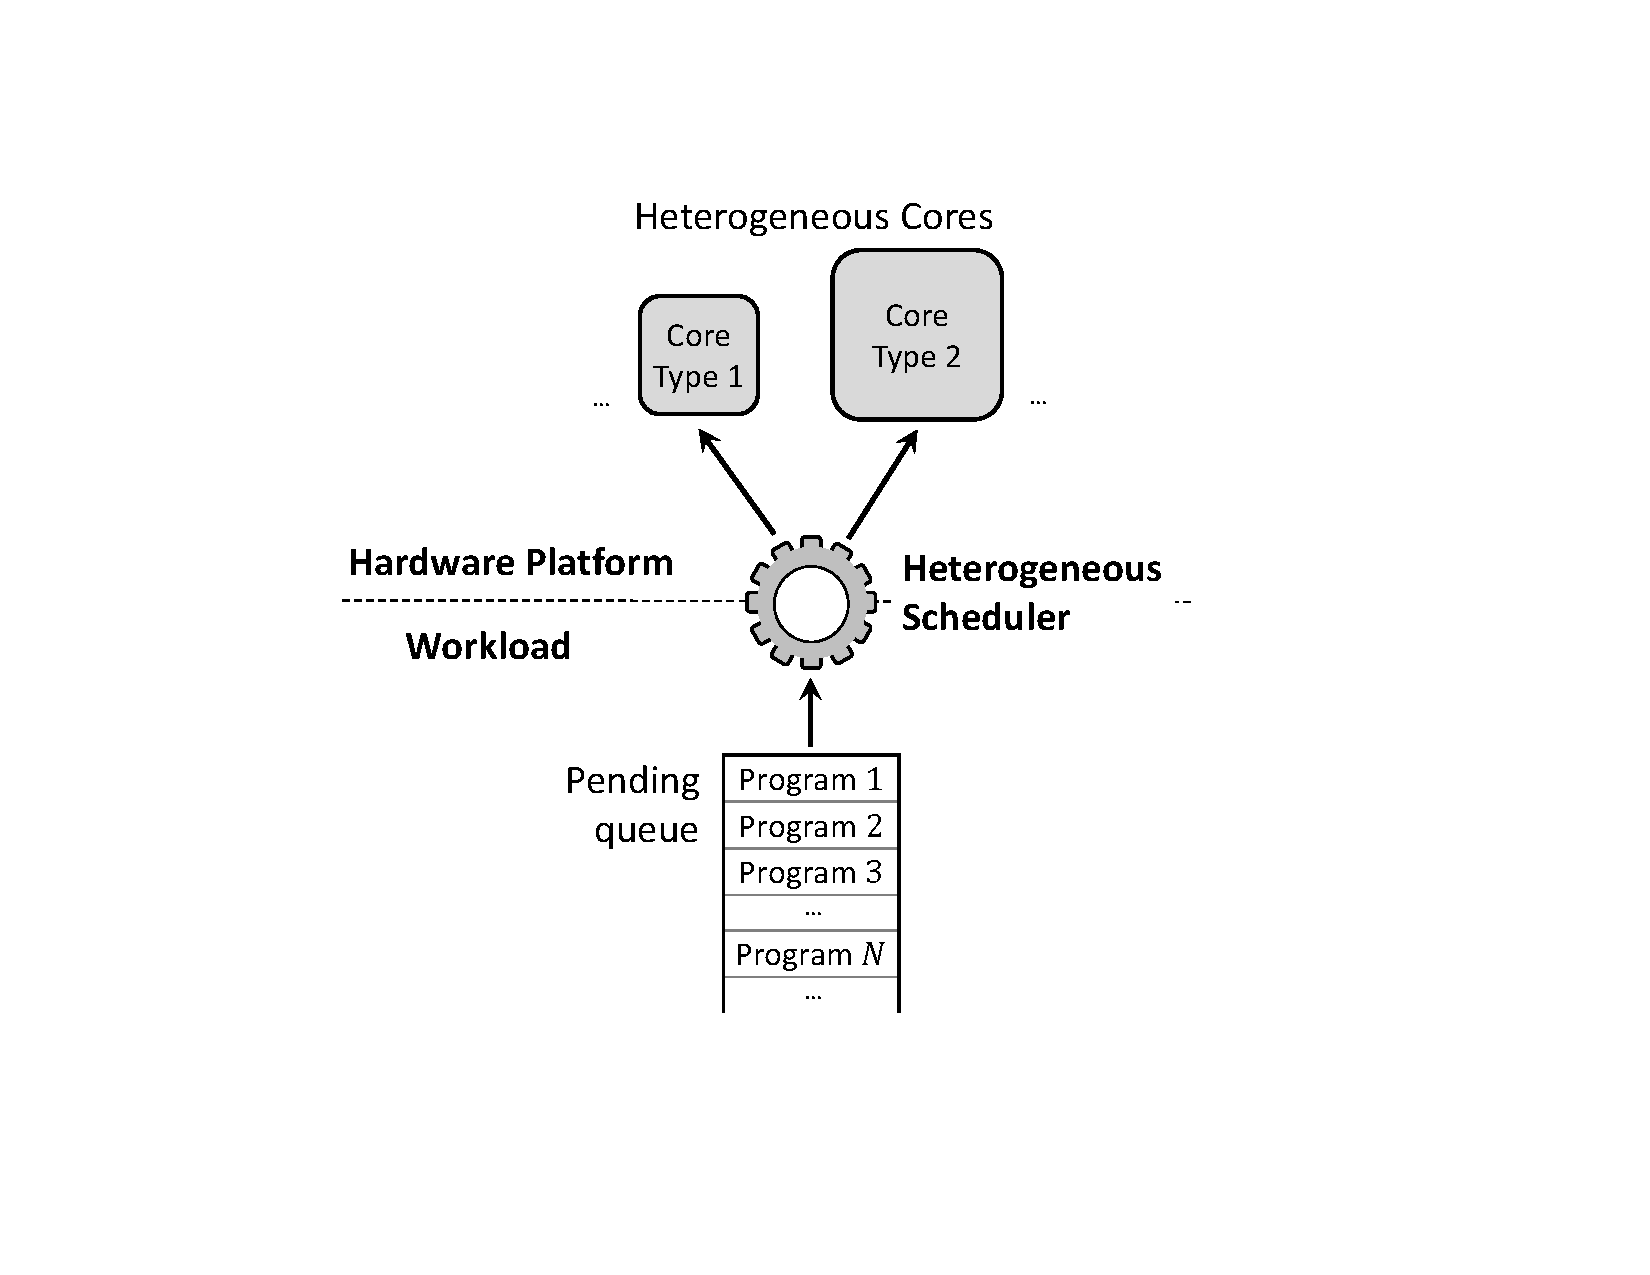
\includegraphics[width=0.5\columnwidth]{figs/heteroExampleOverview.pdf}
\caption{Ключевые компоненты гетерогенного планирования}
\label{fig:heteroExampleOverview}
\end{figure}

\begin{table}
\centering
\captionsetup{justification=centering}
\caption{Требования исполнения программ по их блокам}
\label{tab:demandExample}
\begin{tabular}{|c|c|c|c|c|c|}
\hline
\multicolumn{2}{|c|}{\multirow{2}{*}[-1ex]{\makecell{Программы \\ Блоки}}} & \multicolumn{2}{c|}{Время, сек} & \multicolumn{2}{c|}{Энергия, Джоули} \\[2pt] \cline{3-6}
\multicolumn{2}{|c|}{} & \makecell{Ядро 1 \\ (медленное)} & \makecell{Ядро 2 \\ (быстрое)} & Ядро 1 & Ядро 2 \\ \hline
\multirow{2}{*}{P1} & B1 & 4 & 3 & 8 & 9 \\[2pt] %\cline{2-6}
 & B2 & 5 & 3 & 3 & 4 \\[2pt] \hline
\multirow{3}{*}{P2} & B1 & 5 & 4 & 6 & 10 \\[2pt] %\cline{2-6}
 & B2 & 3 & 2 & 3 & 7 \\[2pt] %\cline{2-6}
 & B3 & 3 & 2 & 3 & 6 \\[2pt] \hline
P3 & B1 & 3 & 2 & 6 & 7 \\[2pt] %\hline
 \hline
\end{tabular}
\end{table}

\begin{figure*}
\begin{subfigure}{.85\columnwidth}
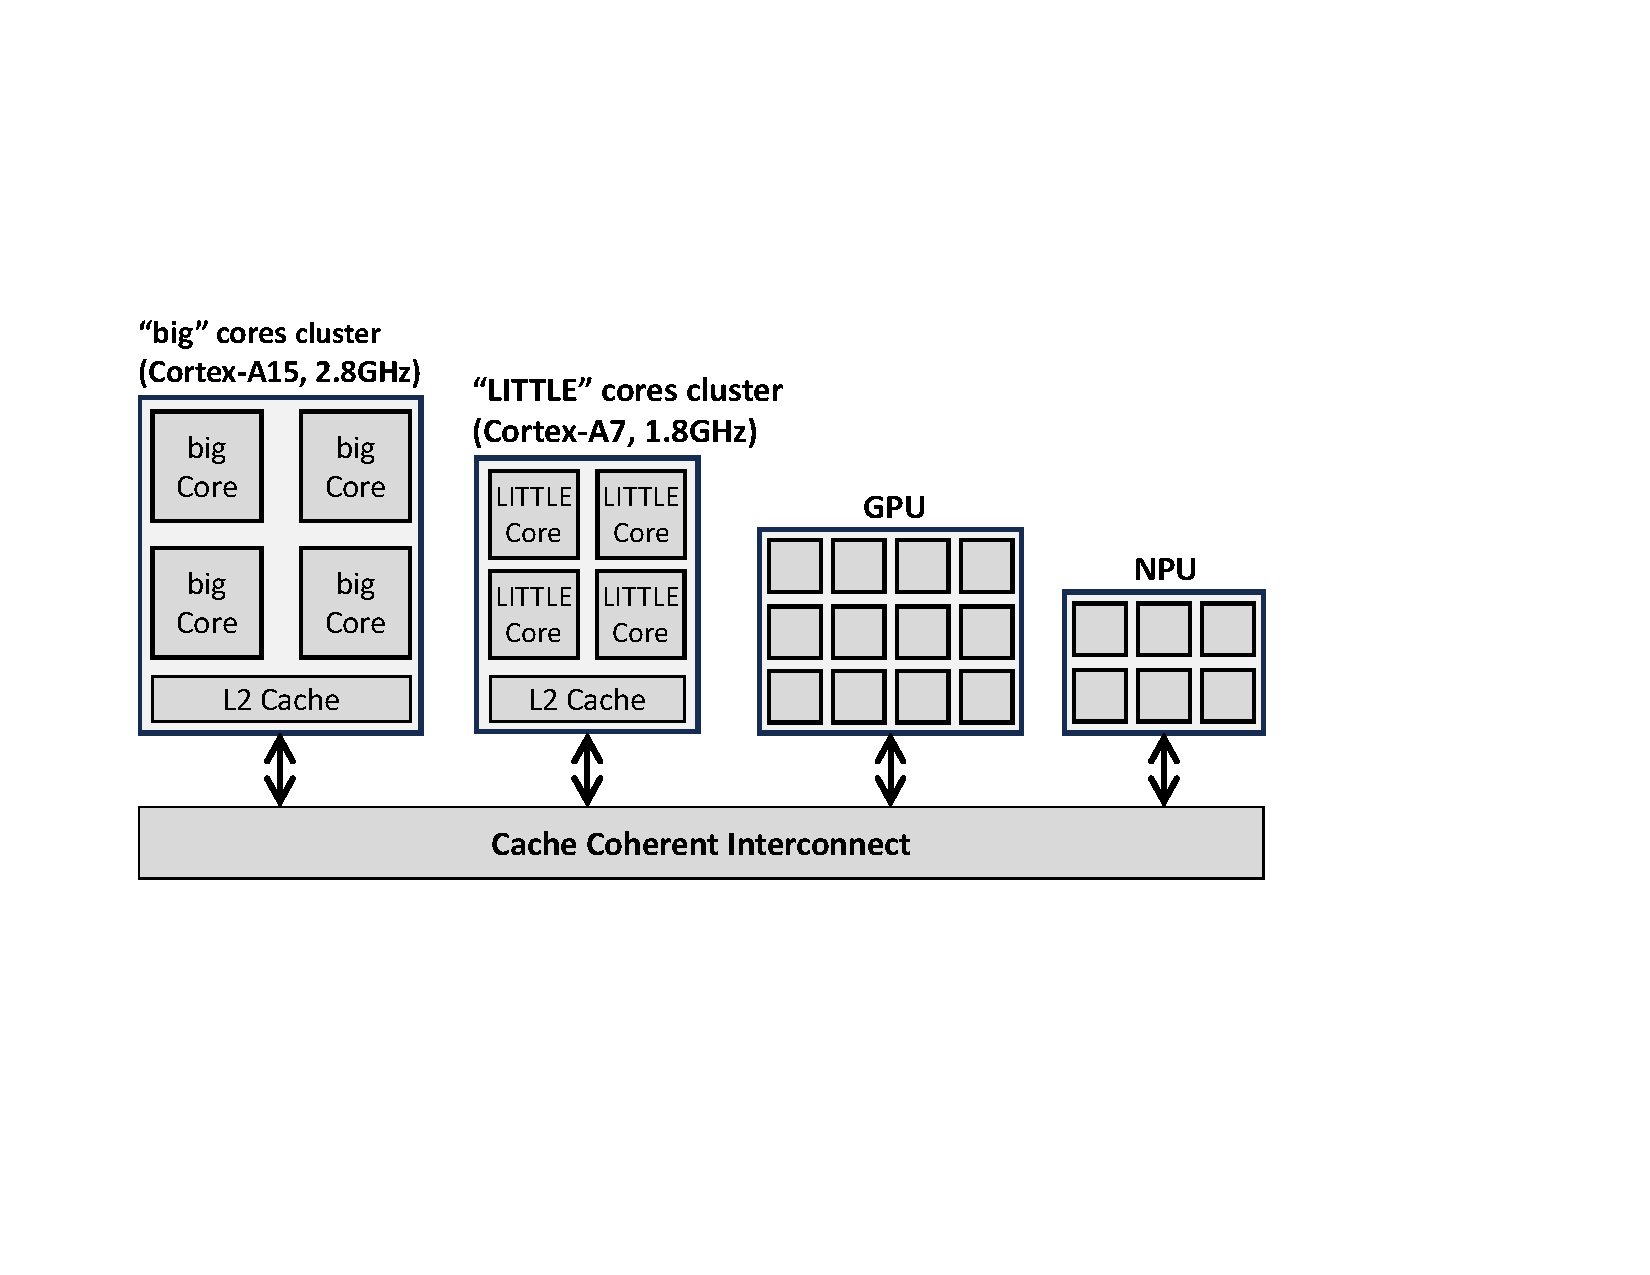
\includegraphics[width=1\linewidth]{figs/bigLITTLEArchitecture.pdf}
\vspace{1mm}
\caption{ARM big.LITTLE архитектура: обзор}
\label{fig:bigLITTLEArchitecture}
\end{subfigure}

\begin{subfigure}{.95\columnwidth}
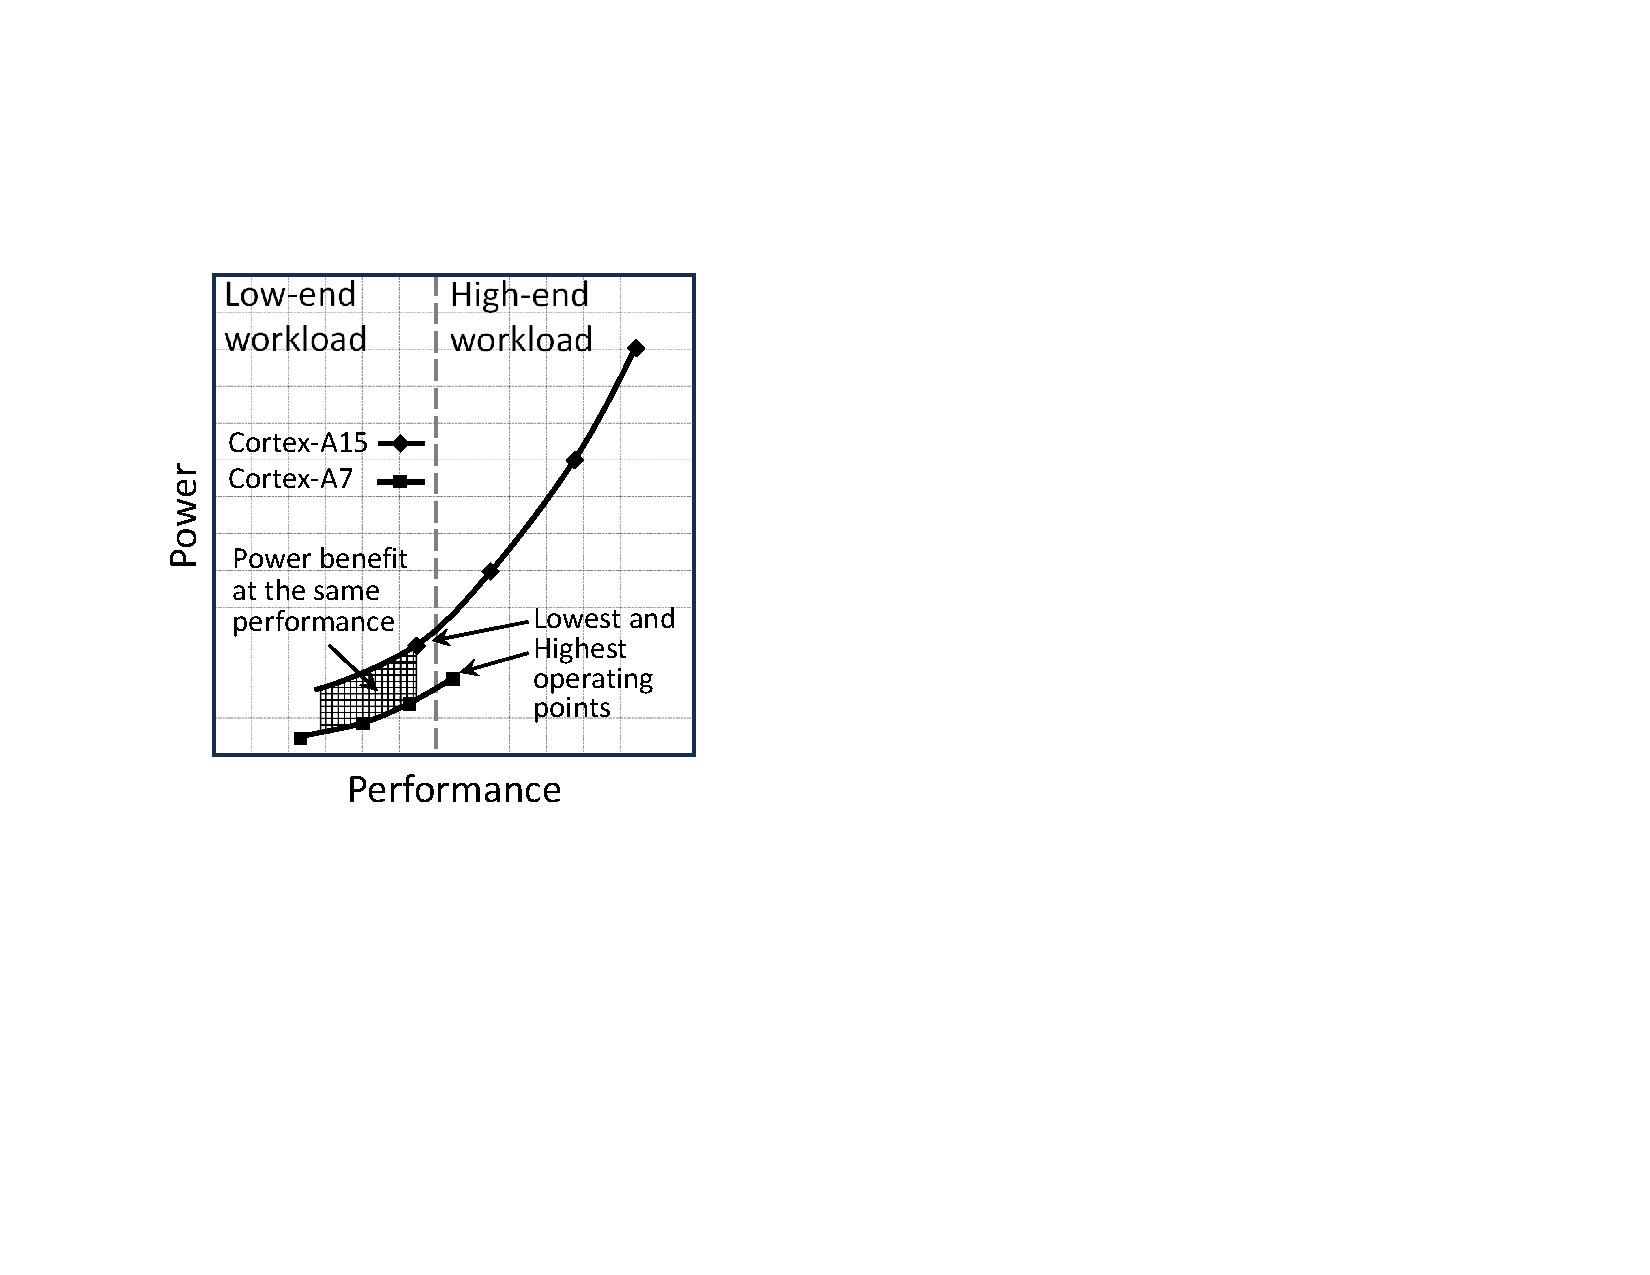
\includegraphics[width=.4\linewidth]{figs/CortexA15vsA7Comparison.pdf}
\vspace{1mm}
\caption{Тренды в производительности и энергопотреблении}
\label{fig:CortexA15A7Comparison}
\end{subfigure}
\caption{Гетерогенная архитектура: пример Cortex-A15 и Cortex-A7}
\end{figure*}

\begin{figure}
\centering
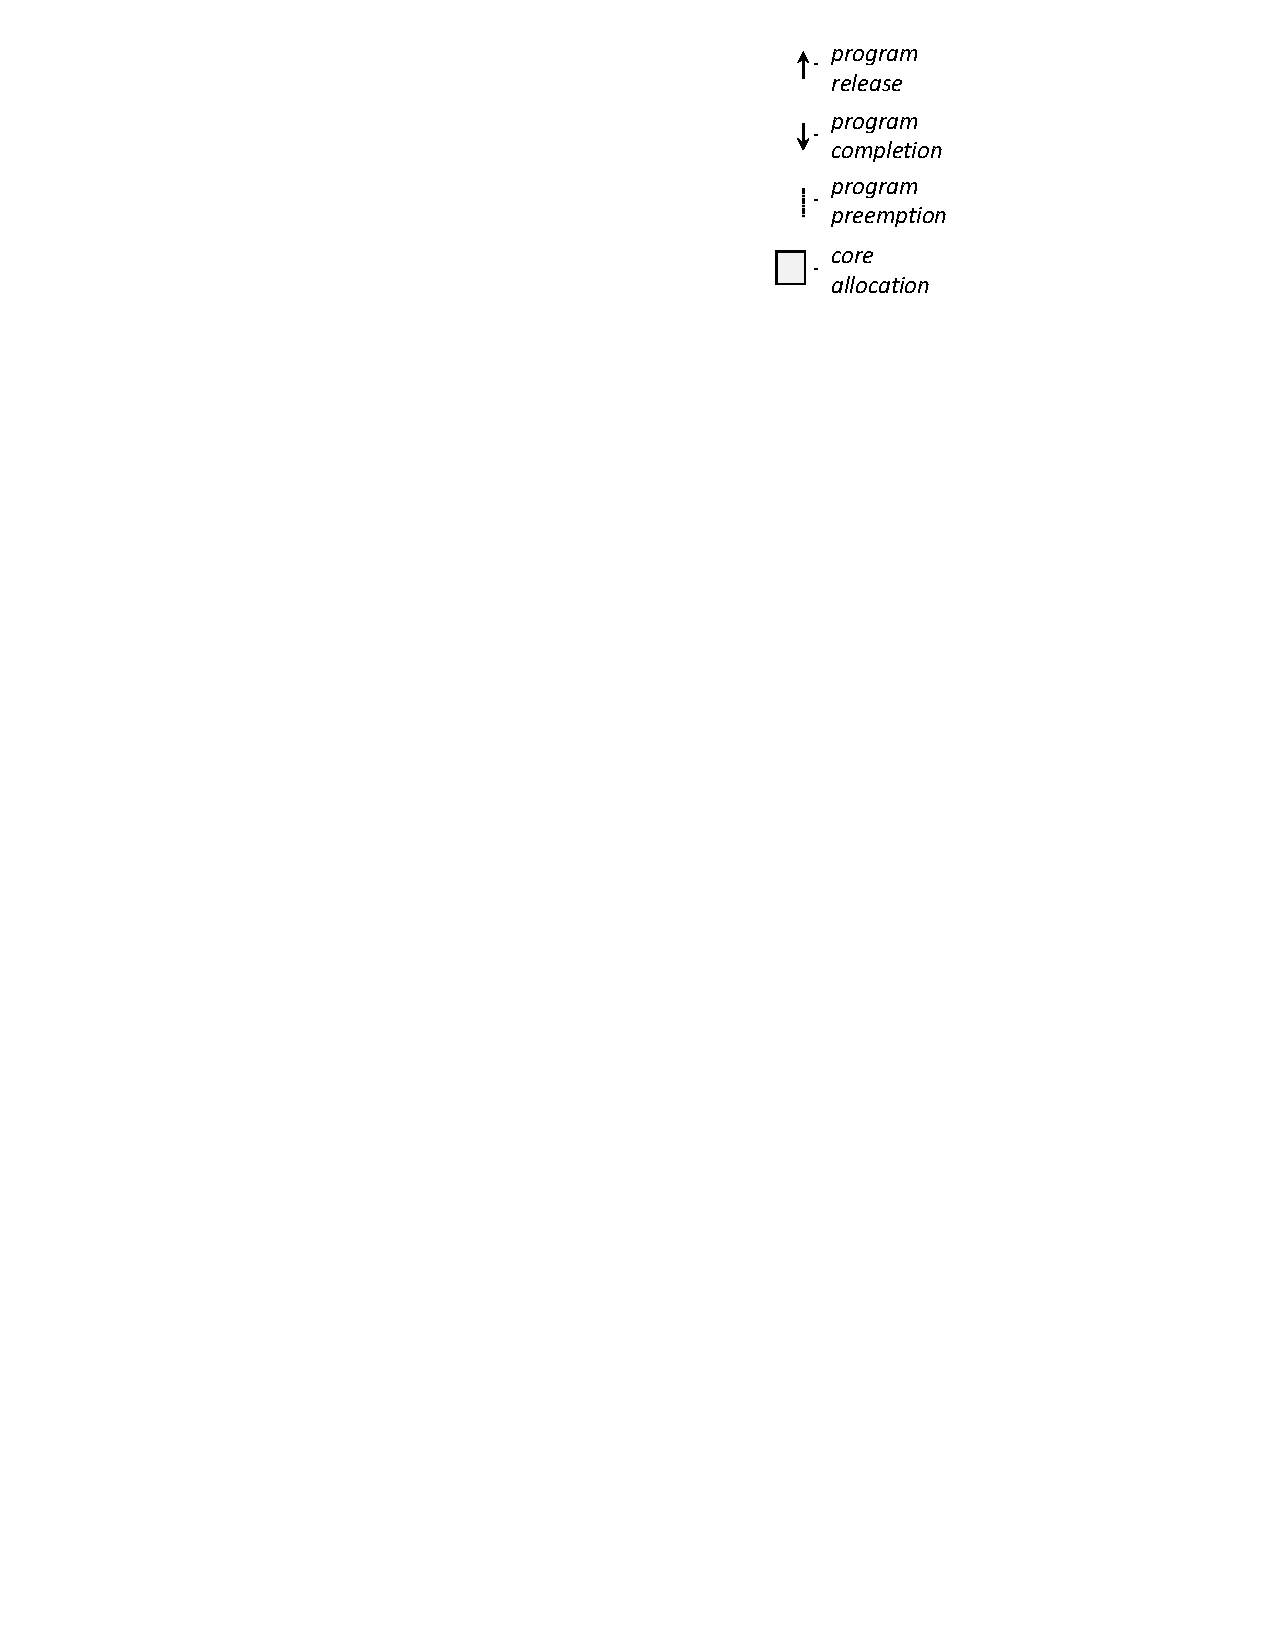
\includegraphics[width=.18\columnwidth]{figs/notation.pdf}
\caption{Графическая нотация}
\label{fig:notation}
\end{figure}


Рисунки, как и остальная часть работы, опираются на графические обозначения, приведенные на рис.~\ref{fig:notation}.

\begin{figure*}
\begin{minipage}{.7\columnwidth}%
\begin{subfigure}{\linewidth}
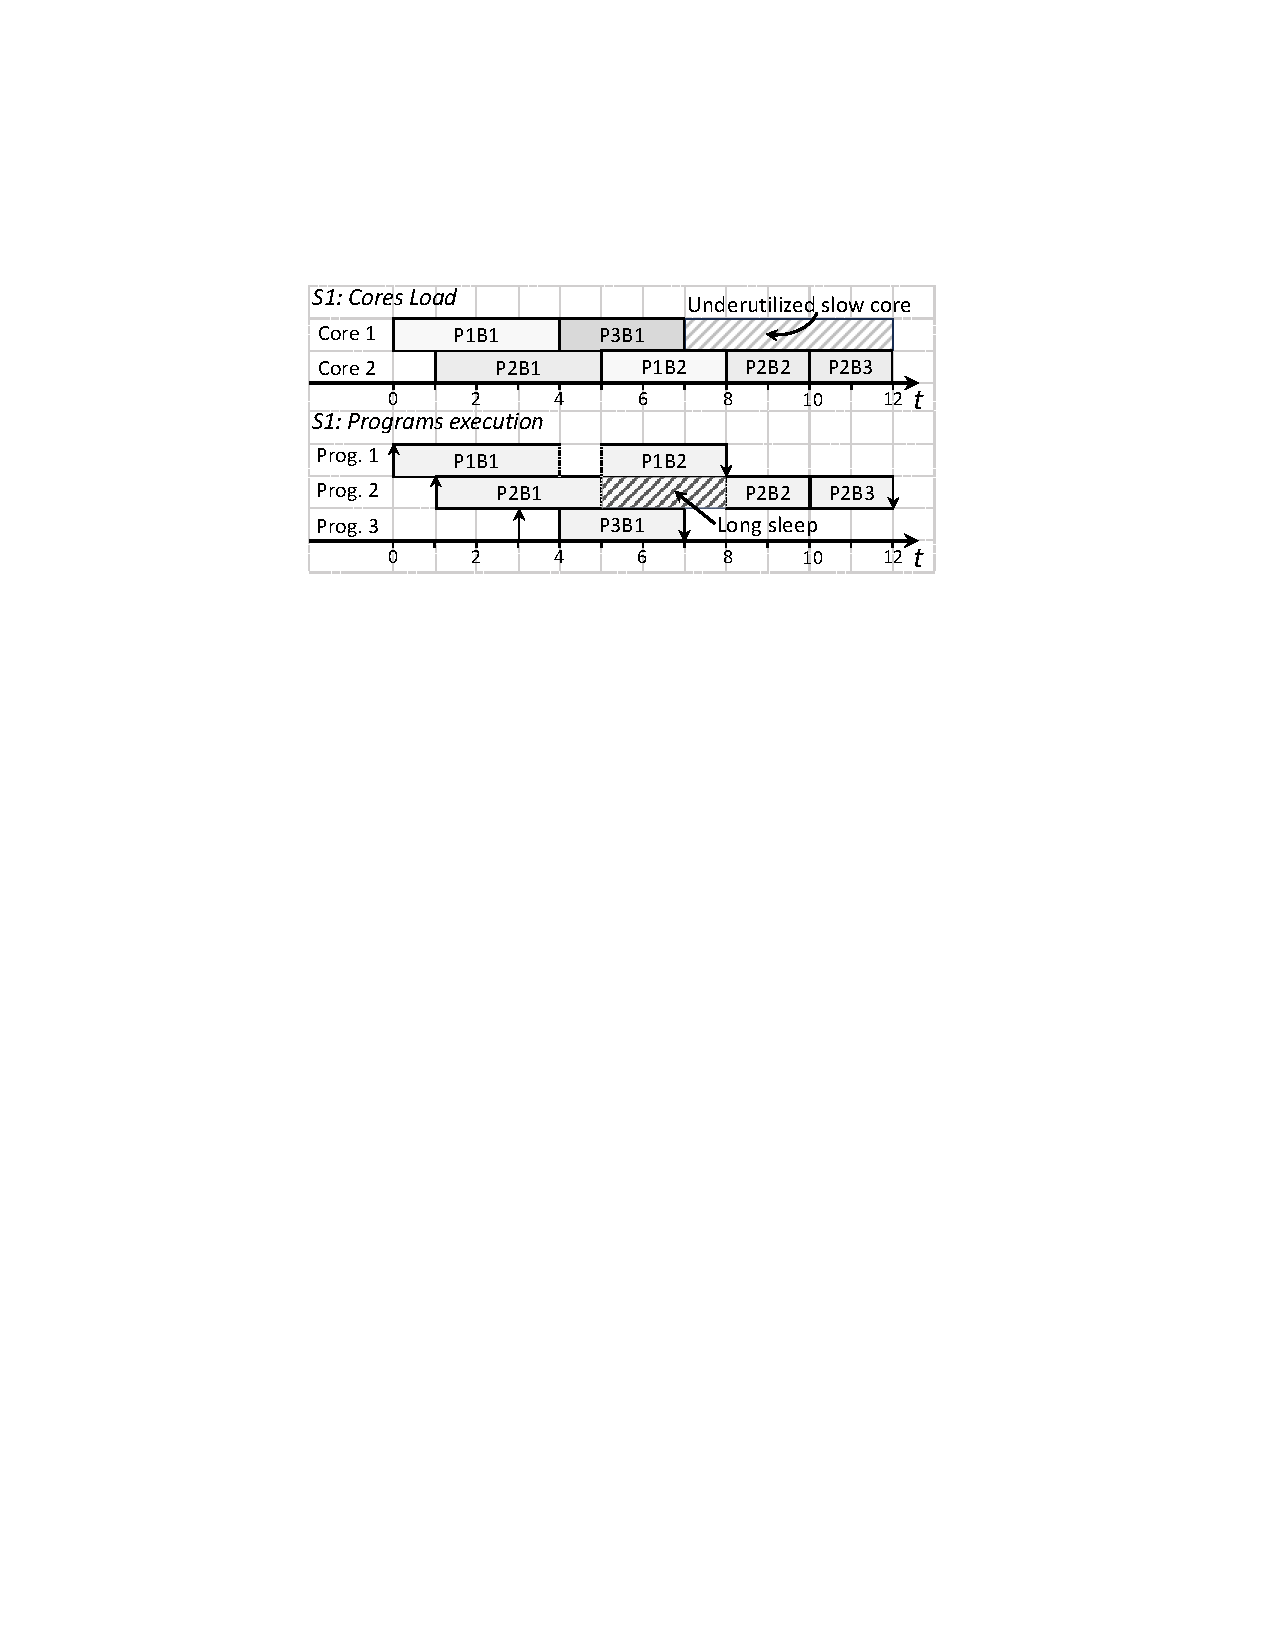
\includegraphics[width=\linewidth]{figs/s1.pdf}
\caption{Schedule S1: исполнение программ}
\vspace{3mm}
\label{fig:s1}
\end{subfigure}

\begin{subfigure}{\linewidth}
\centering
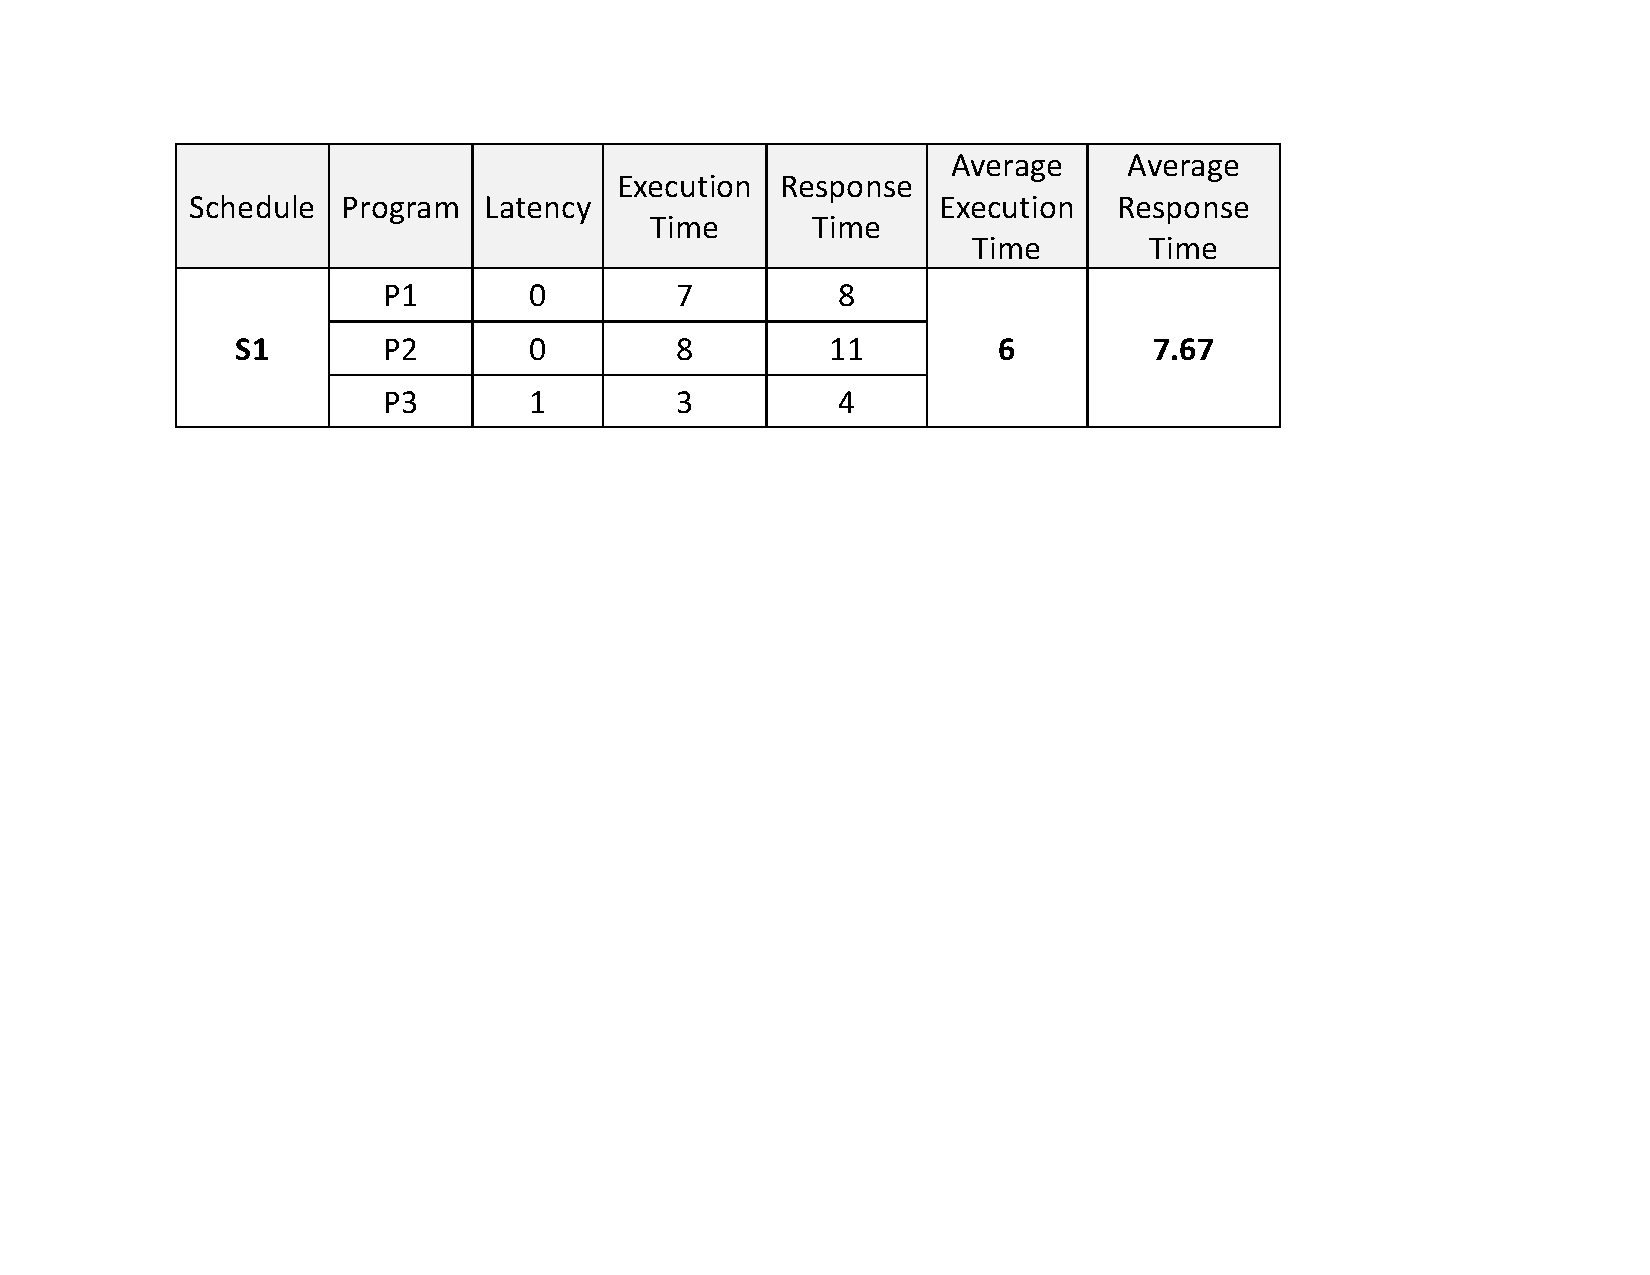
\includegraphics[width=\linewidth]{figs/s1Metrics.pdf}
\caption{S1: временные метрики}
\vspace{1mm}
\label{fig:s1Metrics}
\end{subfigure}
\end{minipage}

\begin{minipage}{.7\columnwidth}%
\begin{subfigure}{\linewidth}
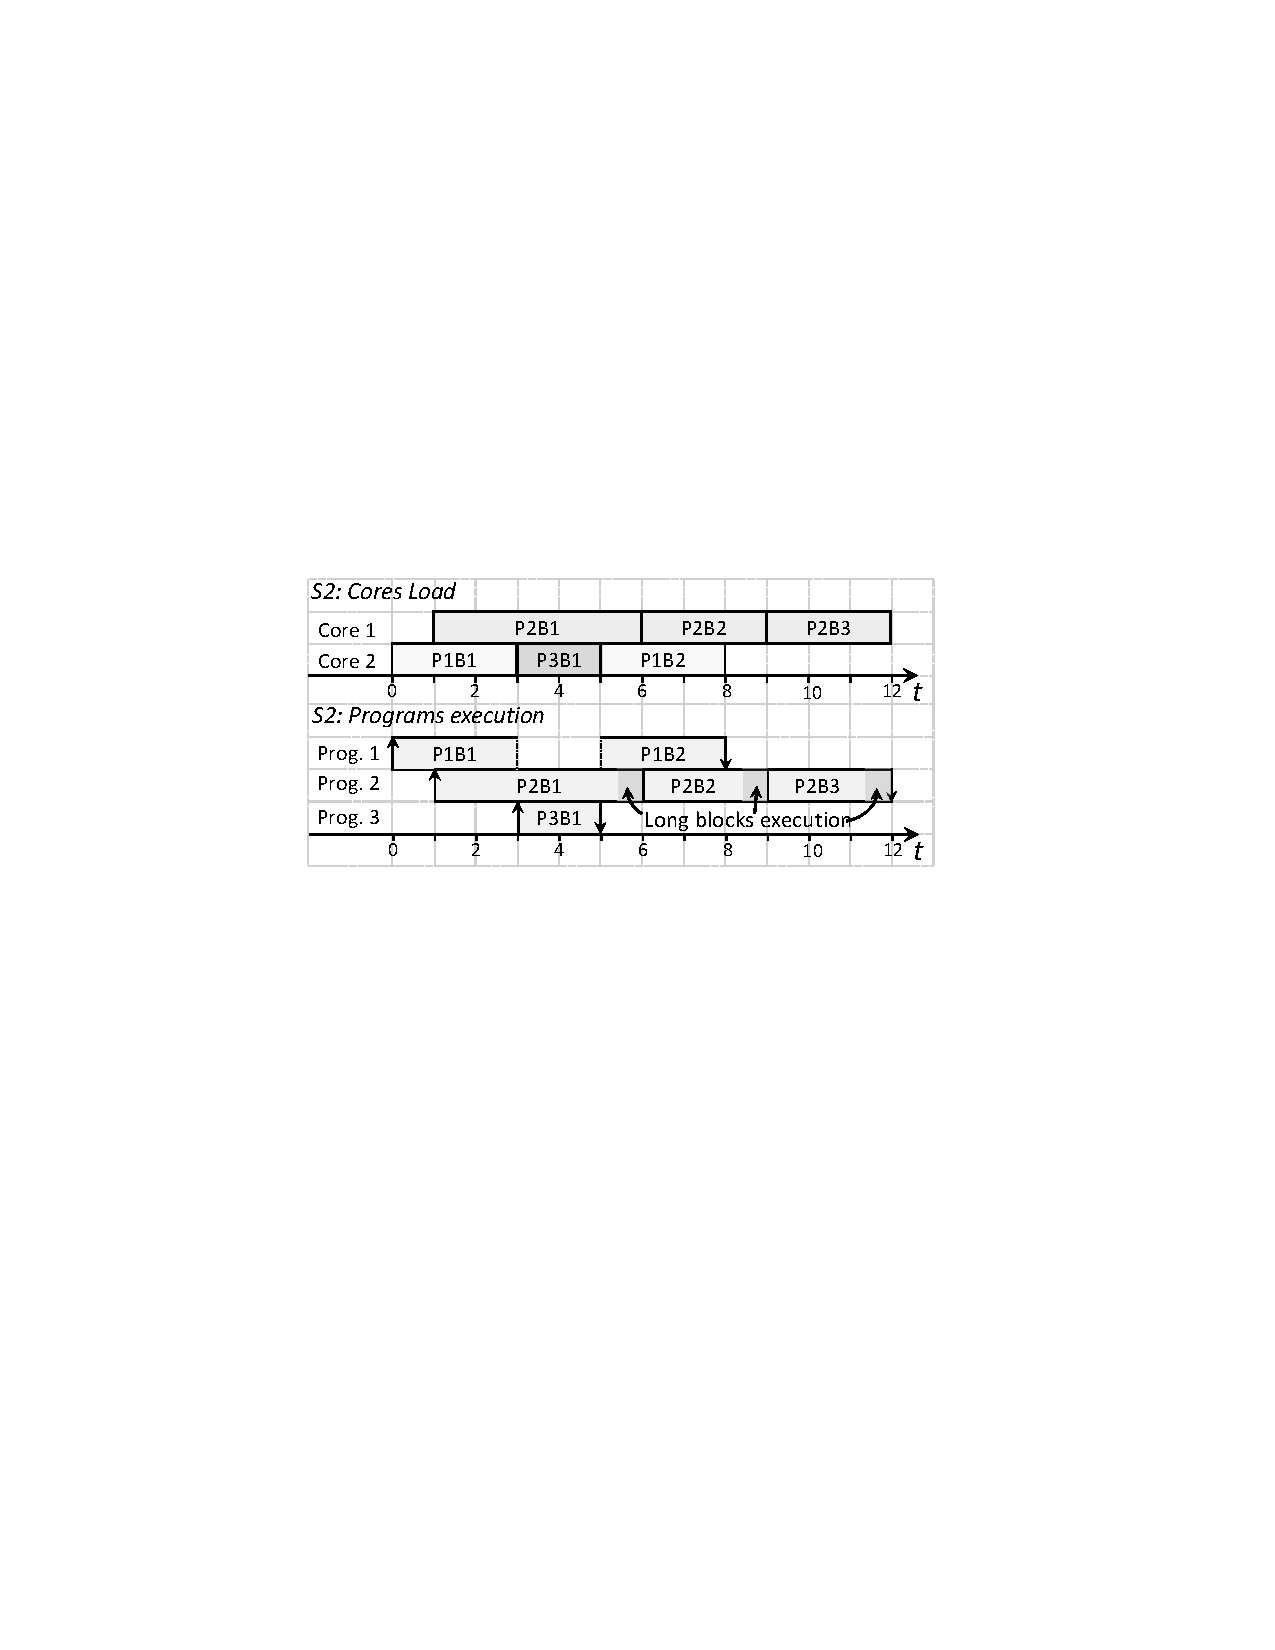
\includegraphics[width=\linewidth]{figs/s2.pdf}
\caption{Schedule S2: исполнение программ}
\vspace{3mm}
\label{fig:s2}
\end{subfigure}

\begin{subfigure}{\linewidth}
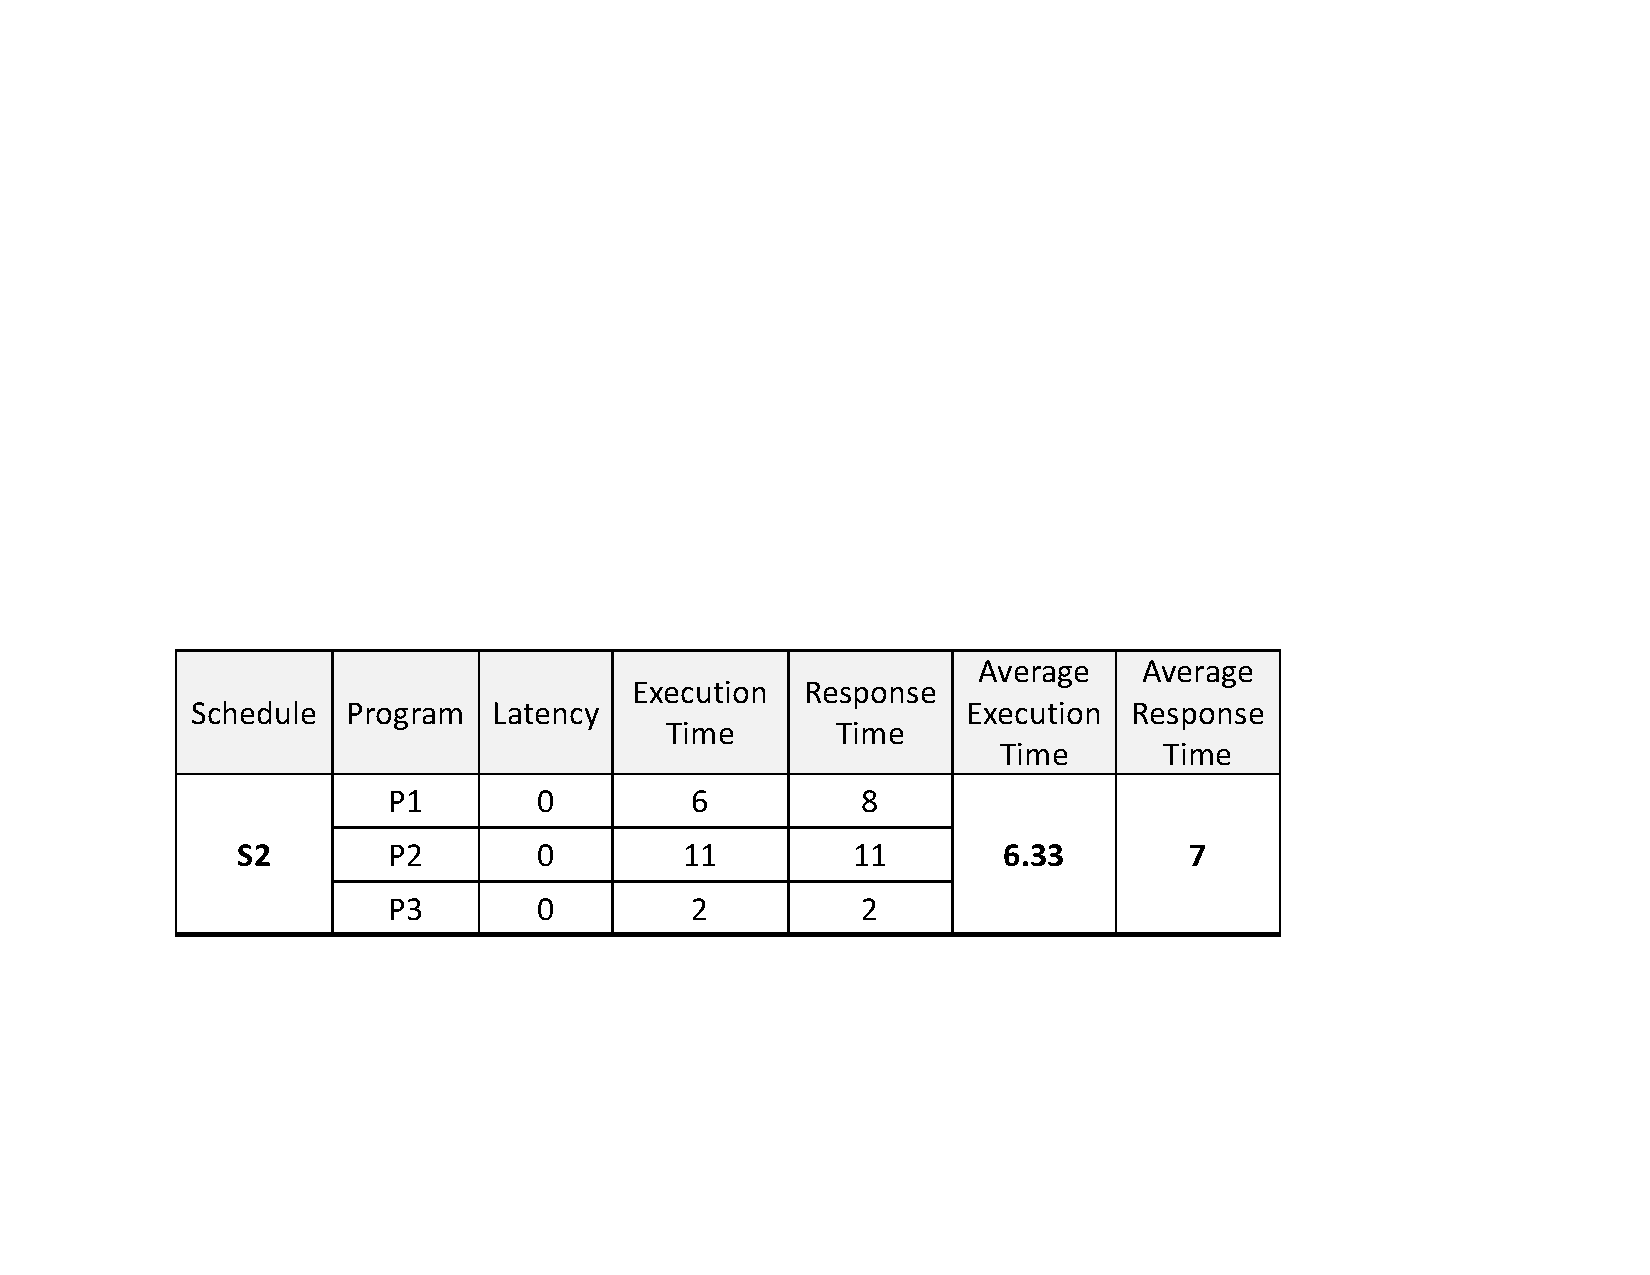
\includegraphics[width=\linewidth]{figs/s2Metrics.pdf}
\caption{S2: временные метрики}
\vspace{1mm}
\label{fig:s2Metrics}
\end{subfigure}
\end{minipage}%

\caption{Примеры планирования программ для требований из таблицы~\ref{tab:demandExample} (миграции и преемственность не учтены)}
\label{fig:twoSchedulesExample}
\vspace{-3mm}
\end{figure*}




















